\documentclass[12pt]{article}

\usepackage{graphicx}
\usepackage{paralist}
\usepackage{amsfonts}
\usepackage{amsmath}
\usepackage{hhline}
\usepackage{booktabs}
\usepackage{multirow}
\usepackage{multicol}
\usepackage{url}
\usepackage{hyperref}

\oddsidemargin -10mm
\evensidemargin -10mm
\textwidth 160mm
\textheight 200mm
\renewcommand\baselinestretch{1.0}

\pagestyle {plain}
\pagenumbering{arabic}

\newcounter{stepnum}

%% Comments

\usepackage{color}

\newif\ifcomments\commentstrue

\ifcomments
\newcommand{\authornote}[3]{\textcolor{#1}{[#3 ---#2]}}
\newcommand{\todo}[1]{\textcolor{red}{[TODO: #1]}}
\else
\newcommand{\authornote}[3]{}
\newcommand{\todo}[1]{}
\fi

\newcommand{\wss}[1]{\authornote{blue}{SS}{#1}}

\title{Assignment 4, Specification}
\author{Hosty Khurana, Khurah2}

\begin {document}

\maketitle
This Module Interface Specification (MIS) document contains modules, types and
methods for implementing the game \textit{2048}. At the start of each game,there occur two random numbers on the command line in a matrix of 4 X 4, the numbers are randomized between 2 or 4 with a 10\% chance that a 4 can occur. There are certain operations that could be applied by the user to play this game which include going up,down,left or right depending on the requirement at that time. The goal of this game is to achieve a 2048 on any of the tile by performing the mentioned operations. The rules of the game are :\\
\begin{itemize}
  \item  When two tiles with the same number on them collide with one another as you move them, they will merge into one tile with the sum of the numbers written on them initially.
 \item A random number(a 2 or a 4) pops up everytime you perform the mentioned operations only if there exist a tile with value Zero(Empty Time).
 \end{itemize} The game can be launched and play by typing \texttt{make run} in terminal.


% In applying the specification, there may be cases that involve undefinedness.
% We will interpret undefinedness following~\cite{Farmer2004}:

% If $p: \alpha_1 \times .... \times \alpha_n \rightarrow \mathbb{B}$ and any of
% $a_1, ..., a_n$ is undefined, then $p(a_1, ..., a_n)$ is False.  For instance,
% if $p(x) = 1/x < 1$, then $p(0) = \text{False}$.  In the language of our
% specification, if evaluating an expression generates an exception, then the
% value of the expression is undefined.

% \wss{The parts that you need to fill in are marked by comments, like this one.
%   In several of the modules local functions are specified.  You can use these
%   local functions to complete the missing specifications.}

% \wss{As you edit the tex source, please leave the \texttt{wss} comments in the
%   file.  Put your answer \textbf{after} the comment.  This will make grading
%   easier.}

% \bibliographystyle{plain}
% \bibliography{SmithCollectedRefs}


\newpage

\section* {View Module}

\subsection*{Template Module}

View

\subsection* {Uses}

None

\subsection* {Syntax}

\subsubsection* {Exported Constants}

None

\subsubsection* {Exported Types}

None

\subsubsection* {Exported Access Programs}

\begin{tabular}{| l | l | l | p{5cm} |}
\hline
\textbf{Routine name} & \textbf{In} & \textbf{Out} & \textbf{Exceptions}\\
\hline
new View & & View & ~\\
\hline
runGame & & & ~\\
\hline
Instructions & & & ~\\
\hline
\end{tabular}

\subsection* {Semantics}

\subsubsection* {State Variables}

$\mathit{gameBoard}: \text{Model}$\\
$\mathit{scanner}: \text{Scanner}$\\
$\mathit{continueGame}: \mathbb{B}$

\subsubsection* {State Invariant}

None

\subsubsection* {Assumptions}

None

\subsubsection* {Access Routine Semantics}

\noindent new View():
\begin{itemize}
\item transition: $\mathit{gameBoard}, \mathit{scanner}, \mathit{continueGame} := \text{new Model}, \text{new Scanner}, \text{true} $
\item output: none
\item exception: none
\end{itemize}

\noindent runGame():
\begin{itemize}
\item transition: Method for running the game. The game starts by displaying a welcome message and 
\item exception: none
\end{itemize}

\noindent Instructions():
\begin{itemize}
\item transition: Displays Welcome Message and rules when user first runs the game. While continueGame variable stays true, it asks the user for a character to make the corresponding move. After every move it checks if the user won or lose the game.\\\\
\begin{tabular}{| l | l |}
\hline
\textbf{Input Char} & \textbf{Action}\\
\hline
'w' $||$ 'W' & gameBoard.action("Up") \\
\hline
\hline
'a' $||$ 'A' & gameBoard.action("Left") \\
\hline
\hline
's' $||$ 'S' & gameBoard.action("Down") \\
\hline
\hline
'd' $||$ 'D' & gameBoard.action("Right") \\
\hline
\hline
'e' $||$ 'E' & continueGame := false \\
\hline
\hline
'r' $||$ 'R' & gameBoard = new Module() \\
\hline
\end{tabular}

\item exception: none
\end{itemize}

\newpage


\section* {Model Module}

\subsection*{Module}

Model

\subsection* {Uses}

None

\subsection* {Syntax}

\subsubsection* {Exported Constants}

None

\subsubsection* {Exported Types}

None

\subsubsection* {Exported Access Programs}

\begin{tabular}{| l | l | l | p{5cm} |}
\hline
\textbf{Routine name} & \textbf{In} & \textbf{Out} & \textbf{Exceptions}\\
\hline
new Model & & Self & \\
\hline
\hline
newGame & & & \\
\hline
\hline
placeNumber & & & \\
\hline
\hline
isEmpty & & $\mathbb{B}$ & \\
\hline
\hline
rotation & $\mathbb{N}$, $\mathbb{B}$ & & \\
\hline
\hline
action & String & & \\
\hline
\hline
calculateMerge & & & \\
\hline
\hline
checkLucky & & $\mathbb{B}$ & \\
\hline
\hline
checkUnlucky & & $\mathbb{B}$ & \\
\hline
\hline
toString & & String & \\
\hline
\hline
isLucky & & $\mathbb{B}$ & \\
\hline
\hline
isUnlucky & & $\mathbb{B}$ & \\
\hline
\hline
getGame & & int seq[$\mathbb{N}$,$\mathbb{N}$] & \\
\hline
\end{tabular}

\subsection* {Semantics}

\subsubsection* {State Variables}

game: seq of [$\mathbb{N},\mathbb{N}$]\\
randomNumber: Random\\
lucky: $\mathbb{B}$\\
unlucky: $\mathbb{B}$\\

\subsubsection* {State Invariant}

None

\subsubsection* {Assumptions}

None

\subsubsection* {Access Routine Semantics}

\noindent new Model():
\begin{itemize}
\item transition: game, randomNumber, lucky, Unlucky := new int[4][4], new Random, true, false\\
This calls newGame.
\item exception: none
\end{itemize}

\noindent newGame():
\begin{itemize}
  \item transition: choose two different random points for x and y between 0 and 3 (inclusive) then put a 2 or a 4 at two random places. Chance of a 4 occuring is 10 percent.
  \item exception: none
\end{itemize}

\noindent placeNumber():
\begin{itemize}
  \item transition: choose random points for x and y between 0 and 3 (inclusive) then Put a 2 or a 4 at empty random places after an action. Chance of a 4 occuring is 10 percent. 
  \item exception: none
\end{itemize}

\noindent isEmpty():
\begin{itemize}
  \item transition: Traverse game (2D array) to find positions that carry 0, if any one position that have 0 exist then return true else false.
  \item output: $\mathbb{B}$   
  \item exception: none
\end{itemize}

\noindent rotation(int angle, boolean rightRotate):
\begin{itemize}
  \item transition: manipulate the game (2D array) by shifting the values vertically or horizontally. The array moves by $90^*$ angle everytime.
  \item exception: none
\end{itemize}

\noindent action(String move):
\begin{itemize}
  \item transition:\\\\
  \begin{tabular}{| l | l |}
\hline
\textbf{move} & \textbf{Action}\\
\hline
"Up" & rotation(90, false) then calculateMerge then rotation(90, true) \\
\hline
\hline
"Down" & rotation(90, true) then calculateMerge then rotation(90, false) \\
\hline
\hline
"Left" & calculteMerge \\
\hline
\hline
"Right" & rotation(180, true) then calculateMerge() then rotation(180, false) \\
\hline
\end{tabular}     
  \item exception: none
\end{itemize}

\noindent calculateMerge():
\begin{itemize}
  \item transition: basic concepts to add the digits using linkedList.
  \item exception: none
\end{itemize}

\noindent checkLucky():
\begin{itemize}
  \item transition: Traverses game (2D array) to find a place with value 2048, If such place is found return true else return false.
  \item output: $\mathbb{B}$
  \item exception: none
\end{itemize}

\noindent checkUnlucky():
\begin{itemize}
  \item transition: Intialize unlucky to be true. Create a copy of game(2D array) and perform all moves on copy of game and if they are equal unlucky remains same but if they are different unlucky becomes false.
  \item output: $\mathbb{B}$
  \item exception: none
\end{itemize}

\noindent toString():
\begin{itemize}
  \item output: Prints game (2D array) in form of a string.
\end{itemize}

\noindent islucky():
\begin{itemize}
  \item output: return value of lucky
\end{itemize}

\noindent isunlucky():
\begin{itemize}
  \item output: return value of unlucky
\end{itemize}

\noindent getGame():
\begin{itemize}
  \item output: return game (2D array)
\end{itemize}

\newpage
\section*{Critique Of Design}
\begin{itemize}
  \item As the game only runs on command line, this specification miss out the oppurtunity to provide lively experience.\\
  \item This specification doesn't display or store high score and current score of the game, making it difficult for user to track his progress.\\
  \item As this specification demands the user to give commands on the console, it becomes difficult to reach the goal that is to achieve a 2048 on any tile.\\
  \item The dependence of modules on each other shows lack of low coupling.\\
  \item Although this specification obeys the laws of generality there still are some functions like $islucky(), isunlucky()$ that could have been avoided.\\
\end{itemize}

\newpage
\graphicspath{{C:/Users/hp/OneDrive/Desktop}}
\section*{UML Diagram For Assignment 3:}
\begin{center}
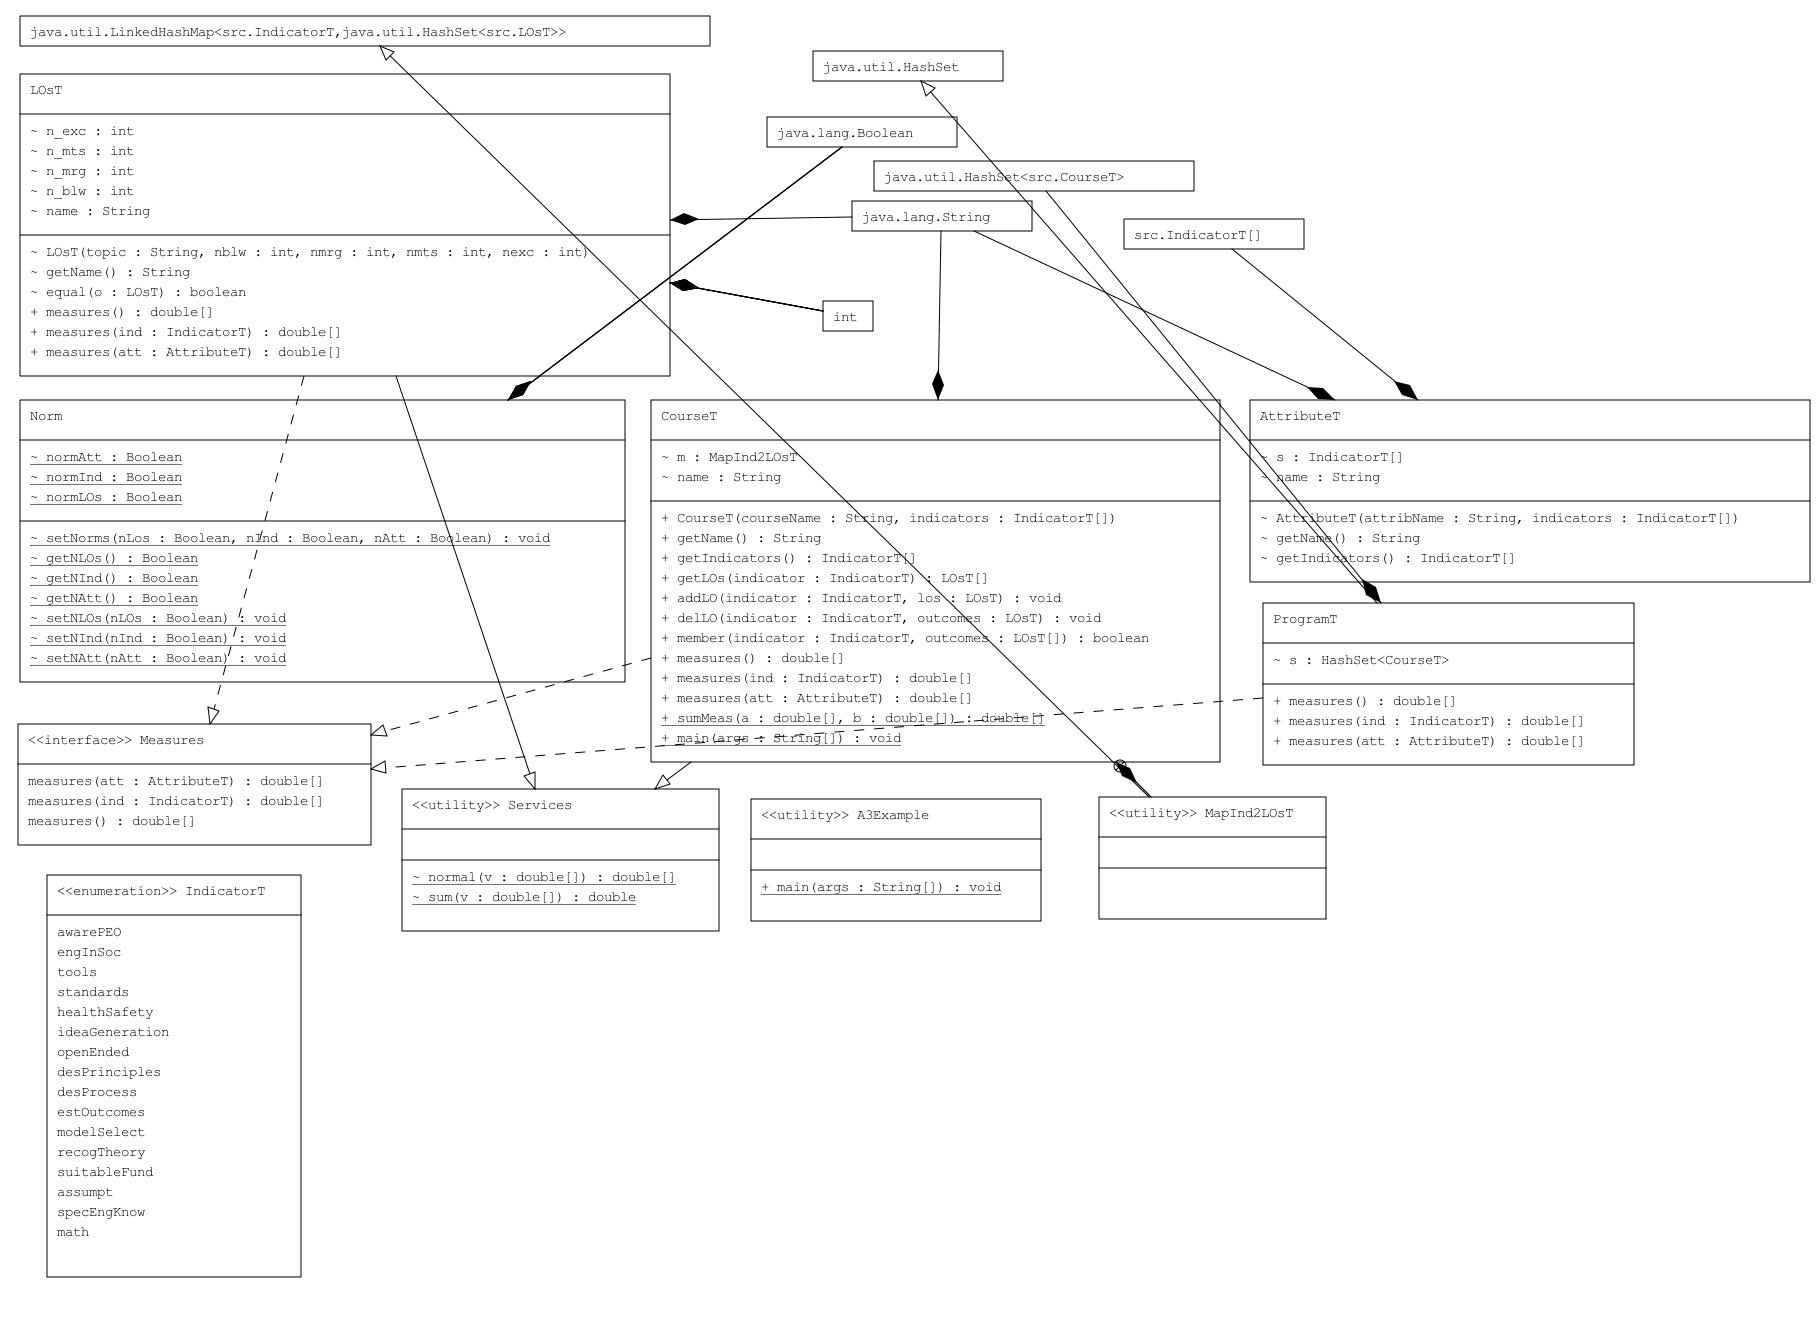
\includegraphics[width=20cm, height=20cm]{UML.png}
\end{center}{}

\end {document}